\section{Dynamic models of ships}

Simple ship dynamic models can be formulated quickly by defining and analyzing the most common propulsion methods. However, these are only vague approximations of the system, and contain few elements of the complex and powerful hydrodynamics.

First the simple ship models are introduced, then an attempt is made to more accurately describe the dynamical system of a ship.

\subsection{Differential drive}

The differential drive system is very common among simple mobile robotic systems. The movement is based on two separately driven wheels placed on either side of the robot body. It can thus change its direction by varying the relative rate of rotation of its wheels, therefore does not require an additional steering mechanism. A twin-screw ship has a somewhat similar layout. Using the engines positioned in a lateral offset to the centerline of the body, the ship can create a torque and propelling force affecting the body.

\begin{figure}[H]
	\centering
	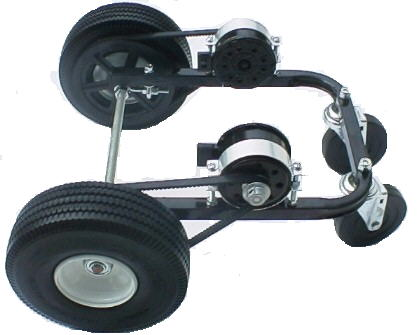
\includegraphics[width=0.8\textwidth]{pics/kadtronixframe}
	\caption{Differential drive robot frame \\ http://www.kadtronix.com/}
	\label{fig:kadtronixframe}
\end{figure}

This type of ship can be modeled as a 2-DOF mobile robot (frame fixed to the body of the ship).

The dynamical system of the parallel propulsion engines can be formulated easily:


Figure here! d is the distance of the wheel from the center

\begin{align}
	\dot{x} &= \frac{v_1}{2} + \frac{v_2}{2} \\
    \dot{\Theta} &= \frac{v_1-v_2}{2*d}
\end{align}

From a control engineer’s point of view the most important aspect of this control system is its linearity. Designing a basic controller for this type of robot is a walk in the park.

The mechanical advantage of this layout is the very high reliability, because the propellers are fixed in a certain angle, therefore they can be build more roboustly, thus decreasing the chance of physical failture. Another advantage is the ability of the ship to turn around it’s central axis, enabling precise maneuvering, however, this is seldom used, because it’s very ineffective with ships.
Usually older large container-ships employ this type of propulsion. Newer large-scale ship design have kept the multi-screw layout, but also included a rudder directly after the propellers to enhance turning.

\subsection{Rudder ship}

The rudder is a controllable part of the ship, creating a tourque on the body of the ship, using hydrodynamical effects, much like the rudders of airplanes. The generated torque depends on the traveling speed. The ship can not rotate around it’s center axis.

The rudder ship can be modeled as a car with Euler(?) steering.

\begin{align}
	\dot{x} &= v \\
	\dot{\Theta} &= \frac{v * tan(\Phi)}{L}
\end{align}

This control type is usually fitted on faster ships, exploiting the possibility to create high torques on the body at high speeds, resulting in sharp turns.

\subsection{Sailing ship}

The sailing ship is usually a rudder controlled ship, but it’s possible to alter the course of a sailing vessel by adjusting the sales or tilting the mast (e.g.: windsurfing).
There are many forces affecting the sails and the body of the ship, but it’s way out of the scope of this text to model all of them. However, they can be generalized in two forces, the lift and the drag.

Lift is the force generated on the saild by the wind, affecting paralell with the body of the ship, and drag is the force generated perpendicular to the body of the ship. These forces are greatly and nonlinearly dependent on the strength and direction of the wind, current speed, air pressure, wind shears, local temperature gradiants and a lot of other circumstances.

However, they allow to generalize the system into a 3-dof system after making the following assumptions:

The relative wind is the vectorial subtraction of the velocity from the wind.
The magnitude of the sail drag is a positive definite function of the relative wind.

The assumptions above result in the following statement:
The sum force caused by the wind is never parallel to the body of the ship. A certain amount of drift always occurs during sailing (hence exists the 3rd degree of freedom).

The resulting dynamical system can be formulated:

\begin{align}
		\dot{x} &= v_x
	\\	\dot{y} &= v_y
	\\	\dot{v}_x &= lift - \frac{v_x}{bodydrag_x}
	\\	\dot{v}_y &= drag - \frac{v_y}{bodydrag_y}
	\\	\dot{\Theta} &= \frac{v_x * tan(\Phi)}{L}
\end{align}

\subsection{Complex ship dynamics}

The hydro- and aerodynamic effects have a great impact on the dynamics of a ship. A perfect prediction is hardly possible, but some considerations can be employed in order to predict the behaviour of a real ship.
The ever-changing draught of the ship, the effects of the viscous medium it’s located in, nonlinear hydrodynamic effects on the turbines and the body and much else causes this severe complexity of the dynamics of a ship. Including the effects of the wind on the body of the ship or the rigg, the resulting system is more like a mess than a clear representation.
However, it’s important to partially unravel these mysteries in order to formulate an effective control system.

From now on, however, in order to evaluate the possible control system methods 

\subsection{Environmental model}

In order to estimate the behavior of an object in natural environment, the ambient effects must be estimated first. The two major environmental factors are the effects of the sea and wind. They generate periodic loads that stirs and slowly wears down objects they contact width. An ocean surface is almost never still, as waves carry the memory of distant and past storms for a long way. However, the ever-changing and chaotic surface of the sea is composed of regular waves, each having its own frequency, direction and amplitude.

A simple, but adequately complex irregular wave model\cite[p.~14]{shipsim} can be derived from the basic hydrodynamic principles using superposition of regular waves\cite[p.~19]{hydromechanics}.

\begin{align}
		\zeta (x, y, t) = T + H_s * \sum_{i=1}^{10} (cos(k .* (x .* sin(\chi) + y * cos(\chi)) + \Omega * \omega{_i} * t + \Phi));
\end{align}

\begin{figure}[H]
	\centering
	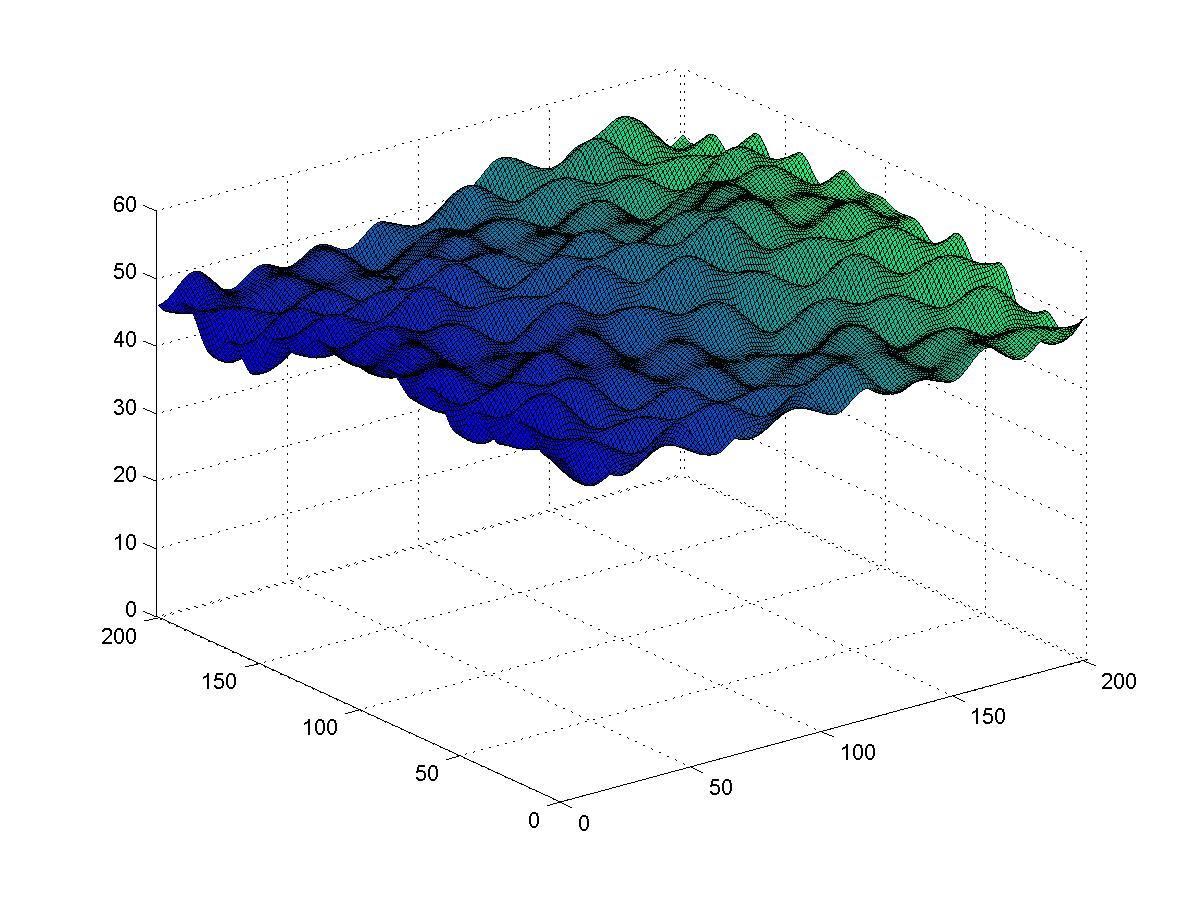
\includegraphics[width=0.8\textwidth]{fig/wavemodel}
	\caption{Simulation result of the irregular wave model}
	\label{fig:wavemodel}
\end{figure}

\subsection{Behavior of floating objects in water}

\subsection{Building simulation environment}

To test the simulation environment a basic visualization

\begin{tcolorbox}[colback=cyan!5,colframe=cyan!40!black,title=Code: Simulator.py \\ https://www.dropbox.com/s/agron9anslev6xw/Simulator.py]
\begin{minipage}{0,6\textwidth}
According to the guidelines of the seamless simulator, this part of the system has its own distinctive object. Everything related to the simulator and everything that is unknown during the mission is stored and handled here.
\end{minipage}
\begin{minipage}{0,35\textwidth}
\raggedleft

\includegraphics[width=0.8\textwidth]{img/simulatorcode}
\end{minipage}
\end{tcolorbox}

\subsection{Uncontrolled system simulation results}